\documentclass[11pt,tikz,border=2mm]{standalone}
\usepackage{csquotes}
\usepackage[backend=biber,style=numeric,sorting=none]{biblatex}

\providecommand{\FigScale}{1.25}
 
\usepackage{siunitx}
\usepackage{tikz}
\usepackage{fontawesome5}
\usetikzlibrary{decorations.pathmorphing,patterns}
\usetikzlibrary{shapes.geometric, arrows, arrows.meta}
\usetikzlibrary{positioning}
 
\usepackage{amsmath}
 
\usepackage{tikz-3dplot}
\usetikzlibrary{3d}
 
\usepackage[siunitx,american]{circuitikz}
 
\usepackage{pgfplots}
\usepgfplotslibrary{units}
\usepgfplotslibrary{groupplots}
\pgfplotsset{compat=1.14}
 
\ctikzset{tripoles/mos style/arrows}

\definecolor{IBM1}{HTML}{648fff}
\definecolor{IBM2}{HTML}{785ef0}
\definecolor{IBM3}{HTML}{dc267f}
\definecolor{IBM4}{HTML}{fe6100}
\definecolor{IBM5}{HTML}{ffb000}
\definecolor{IBM6}{HTML}{d55e00}
\definecolor{IBM7}{HTML}{cc79a7}
\definecolor{IBM8}{HTML}{0072b2}
\definecolor{IBM9}{HTML}{f0e442}
\definecolor{IBM10}{HTML}{009e73}

\begin{document}

\begin{tikzpicture}[scale=\FigScale, line join=round, line cap=round, line width=0.4pt]

\tikzset{
  coordlegend/.style={coord, minimum size=8mm},
  routerlegend/.style={router, minimum size=8mm},
  enddevlegend/.style={enddev, minimum size=3.5mm},
  coord/.style={circle, fill=IBM10, draw=black!69, minimum size=8mm},
  router/.style={circle, fill=IBM8, draw=black!69, minimum size=8mm},
  enddev/.style={circle, fill=IBM5, draw=black!69, minimum size=3.5mm},
  link/.style={<->,
    >={Stealth[length=2pt,width=1.6pt]},
    line width=0.5pt, shorten <=0.75pt, shorten >=0.75pt, IBM5},
  link2/.style={<->,
    >={Stealth[length=2pt,width=1.6pt]},
    line width=0.5pt, shorten <=0.75pt, shorten >=0.75pt, IBM8},
  link3/.style={<->,
    >={Stealth[length=2pt,width=1.6pt]},
    line width=0.5pt, shorten <=1.35pt, shorten >=1pt, IBM10},
}

\def\bladeScale{0.69}

\path[shade, left color=gray!10, right color=gray!90, draw=black]
	(-0.55,0) -- (0.55,0) -- (0.18,6) -- (-0.18,6) -- (-0.55,0);

\path[fill=gray!69, draw=black] (-0.48,1.2-0.08) -- (-0.471,1.2+0.08) -- (0.471,1.2+0.08) -- (0.48,1.2-0.08) -- cycle;
    \path[fill=black, draw=black] (-0.4,1.2) circle (0.04);
    \path[fill=black, draw=black] (-0.2,1.2) circle (0.04);
    \path[fill=black, draw=black] (0,1.2) circle (0.04);
    \path[fill=black, draw=black] (0.2,1.2) circle (0.04);
    \path[fill=black, draw=black] (0.4,1.2) circle (0.04);
    
    \path[fill=IBM5, draw=IBM5] (-0.4,1.2) circle (0.02);
    \path[fill=IBM5, draw=IBM5] (-0.2,1.2) circle (0.02);
    \path[fill=IBM5, draw=IBM5] (0,1.2) circle (0.02);
    \path[fill=IBM5, draw=IBM5] (0.2,1.2) circle (0.02);
    \path[fill=IBM5, draw=IBM5] (0.4,1.2) circle (0.02);
    
    \node[circle, minimum size=0.08cm, inner sep=0pt, outer sep=0pt, draw=none, fill=none] (r1e1) at (-0.4,1.2) {};
    \node[circle, minimum size=0.08cm, inner sep=0pt, outer sep=0pt, draw=none, fill=none] (r1e2) at (-0.2,1.2) {};
    \node[circle, minimum size=0.08cm, inner sep=0pt, outer sep=0pt, draw=none, fill=none] (r1e3) at (0,1.2) {};
    \node[circle, minimum size=0.08cm, inner sep=0pt, outer sep=0pt, draw=none, fill=none] (r1e4) at (0.2,1.2) {};
    \node[circle, minimum size=0.08cm, inner sep=0pt, outer sep=0pt, draw=none, fill=none] (r1e5) at (0.4,1.2) {};

    \path[fill=IBM8, draw=IBM8] (0,1.5) circle (0.1);
      \node[circle, minimum size=0.2cm, inner sep=0pt, outer sep=0pt, draw=none, fill=none] (r1) at (0,1.5) {};

    
\path[fill=gray!69, draw=black] (-0.37,3-0.08) -- (-0.36,3+0.08) -- (0.36,3+0.08) -- (0.37,3-0.08) -- cycle;
    \path[fill=black, draw=black] (-0.29,3) circle (0.04);
    \path[fill=black, draw=black] (-0.093333,3) circle (0.04);
    \path[fill=black, draw=black] (0.093333,3) circle (0.04);
    \path[fill=black, draw=black] (0.29,3) circle (0.04);
    
    \path[fill=IBM5, draw=IBM5] (-0.29,3) circle (0.02);
    \path[fill=IBM5, draw=IBM5] (-0.093333,3) circle (0.02);
    \path[fill=IBM5, draw=IBM5] (0.093333,3) circle (0.02);
    \path[fill=IBM5, draw=IBM5] (0.29,3) circle (0.02);

    \node[circle, minimum size=0.08cm, inner sep=0pt, outer sep=0pt, draw=none, fill=none] (r2e1) at (-0.29,3) {};
    \node[circle, minimum size=0.08cm, inner sep=0pt, outer sep=0pt, draw=none, fill=none] (r2e2) at (-0.093333,3) {};
    \node[circle, minimum size=0.08cm, inner sep=0pt, outer sep=0pt, draw=none, fill=none] (r2e3) at (0.093333,3) {};
    \node[circle, minimum size=0.08cm, inner sep=0pt, outer sep=0pt, draw=none, fill=none] (r2e4) at (0.29,3) {};

    \path[fill=IBM8, draw=IBM8] (0,3.3) circle (0.1);
      \node[circle, minimum size=0.2cm, inner sep=0pt, outer sep=0pt, draw=none, fill=none] (r2) at (0,3.3) {};

    
\path[fill=gray!69, draw=black] (-0.259,4.8-0.08) -- (-0.249,4.8+0.08) -- (0.249,4.8+0.08) -- (0.259,4.8-0.08) -- cycle;
    \path[fill=black, draw=black] (-0.179,4.8) circle (0.04);
    \path[fill=black, draw=black] (0,4.8) circle (0.04);
    \path[fill=black, draw=black] (0.179,4.8) circle (0.04);
    
    \path[fill=IBM5, draw=IBM5] (-0.179,4.8) circle (0.02);
    \path[fill=IBM5, draw=IBM5] (0,4.8) circle (0.02);
    \path[fill=IBM5, draw=IBM5] (0.179,4.8) circle (0.02);

    \node[circle, minimum size=0.08cm, inner sep=0pt, outer sep=0pt, draw=none, fill=none] (r3e1) at (-0.179,4.8) {};
    \node[circle, minimum size=0.08cm, inner sep=0pt, outer sep=0pt, draw=none, fill=none] (r3e2) at (0,4.8) {};
    \node[circle, minimum size=0.08cm, inner sep=0pt, outer sep=0pt, draw=none, fill=none] (r3e3) at (0.179,4.8) {};

    \path[fill=IBM8, draw=IBM8] (0,5.1) circle (0.1);
      \node[circle, minimum size=0.2cm, inner sep=0pt, outer sep=0pt, draw=none, fill=none] (r3) at (0,5.1) {};



\begin{scope}[rotate around={30:(0,6.4)}]
  \begin{scope}[shift={(0,6.8)}, scale=\bladeScale, shift={(0,-6.8)}]
    \path[shade, top color=gray!10, bottom color=gray!90, draw=black]
      (0.2,6.8)
      .. controls (0.65,7.51) and (0.45,9.00) .. (0.08,10.8)
      .. controls (0.0,11.04) and (-0.08,11.04) .. (-0.16,10.8)
      .. controls (-0.55,8.92) and (-0.75,7.35) .. (-0.2,6.8)
        -- (0.2,6.8);
  \end{scope}
\end{scope}

\begin{scope}[rotate around={150:(0,6.4)}]
  \begin{scope}[shift={(0,6.8)}, scale=\bladeScale, shift={(0,-6.8)}]
    \path[shade, left color=gray!10, right color=gray!90, draw=black]
      (0.2,6.8)
      .. controls (0.65,7.51) and (0.45,9.00) .. (0.08,10.8)
      .. controls (0.0,11.04) and (-0.08,11.04) .. (-0.16,10.8)
      .. controls (-0.55,8.92) and (-0.75,7.35) .. (-0.2,6.8)
        -- (0.2,6.8);
  \end{scope}
\end{scope}

\begin{scope}[rotate around={270:(0,6.4)}]
  \begin{scope}[shift={(0,6.8)}, scale=\bladeScale, shift={(0,-6.8)}]
    \path[shade, right color=gray!10, left color=gray!90, draw=black]
      (0.2,6.8)
      .. controls (0.65,7.51) and (0.45,9.00) .. (0.08,10.8)
      .. controls (0.0,11.04) and (-0.08,11.04) .. (-0.16,10.8)
      .. controls (-0.55,8.92) and (-0.75,7.35) .. (-0.2,6.8)
        -- (0.2,6.8);
  \end{scope}
\end{scope}

\path[shade, left color=gray!35, right color=gray!55, draw=black] (0,6.4) circle (0.5);

\path[fill=IBM10, draw=IBM10] (-0.3,6.4) circle (0.175);
\coordinate (mc) at (-0.3,6.4) {};
  \node[circle, minimum size=0.35cm, inner sep=0pt, outer sep=0pt, draw=none, fill=none] (mc) at (-0.3,6.4) {};

\node[inner sep=0pt, scale=0.86] at (0.25,6.435) {\faWifi};
    \draw[link3] (-0.15, 6.4) --++ (0.28,0);

% \begin{scope}[shift={(0.07,6.36)},scale=0.2]
%     \draw[semithick] (0,0) rectangle (1.75,1.25);
%         \node[inner sep=0pt, scale=0.69] at (0.875,0.65) {\faWifi};
%     \draw[semithick] (0,-0.1) -- (0,-0.85) -- (1.75,-0.85) -- (1.75,-0.1);
%     \foreach \i in {0.3,0.5,...,1.3} {
%         \draw[ultra thin] (\i,-0.25) rectangle ++(0.1,0.1);
%     }
%     \foreach \i in {0.3,0.5,...,1.3} {
%         \draw[ultra thin] (\i,-0.45) rectangle ++(0.1,0.1);
%     }
%     \foreach \i in {0.3,0.5,...,1.3} {
%         \draw[ultra thin] (\i,-0.65) rectangle ++(0.1,0.1);
%     }    
%     \end{scope}

    \draw[link] (r1) -- (r1e1);
    \draw[link] (r1) -- (r1e2);
    \draw[link] (r1) -- (r1e3);
    \draw[link] (r1) -- (r1e4);
    \draw[link] (r1) -- (r1e5);

    \draw[link] (r2) -- (r2e1);
    \draw[link] (r2) -- (r2e2);
    \draw[link] (r2) -- (r2e3);
    \draw[link] (r2) -- (r2e4);

    \draw[link] (r3) -- (r3e1);
    \draw[link] (r3) -- (r3e2);
    \draw[link] (r3) -- (r3e3);


    \draw[link2] (r1) -- (r2);
    \draw[link2] (r2) -- (r3);
    \draw[link2] (r3) -- (mc);

    \node[coordlegend,
      label={[font=\small]right:Coordinator}] at (-4.5,6.45) {};
    \node[routerlegend,
      label={[font=\small]right:Router}] at (-4.5,4.75) {};
    \node[enddevlegend,
      label={[font=\small]right:End device}] at (-4.5,3.05) {};

\end{tikzpicture}

\end{document}